\documentclass[14pt]{extbook}
\usepackage{multicol, enumerate, enumitem, hyperref, color, soul, setspace, parskip, fancyhdr} %General Packages
\usepackage{amssymb, amsthm, amsmath, latexsym, units, mathtools} %Math Packages
\everymath{\displaystyle} %All math in Display Style
% Packages with additional options
\usepackage[headsep=0.5cm,headheight=12pt, left=1 in,right= 1 in,top= 1 in,bottom= 1 in]{geometry}
\usepackage[usenames,dvipsnames]{xcolor}
\usepackage{dashrule}  % Package to use the command below to create lines between items
\newcommand{\litem}[1]{\item#1\hspace*{-1cm}\rule{\textwidth}{0.4pt}}
\pagestyle{fancy}
\lhead{Progress Quiz 6}
\chead{}
\rhead{Version B}
\lfoot{1430-1829}
\cfoot{}
\rfoot{test}
\begin{document}

\begin{enumerate}
\litem{
Solve the radical equation below. Then, choose the interval(s) that the solution(s) belongs to.\[ \sqrt{8 x^2 + 56} - \sqrt{44 x} = 0 \]\begin{enumerate}[label=\Alph*.]
\item \( x \in [1.81,3.13] \)
\item \( x_1 \in [1.81, 3.13] \text{ and } x_2 \in [-1.5,4.5] \)
\item \( \text{All solutions lead to invalid or complex values in the equation.} \)
\item \( x \in [3.16,4.72] \)
\item \( x_1 \in [-3.78, -3.05] \text{ and } x_2 \in [-4,-0] \)

\end{enumerate} }
\litem{
What is the domain of the function below?\[ f(x) = \sqrt[4]{3 x + 4} \]\begin{enumerate}[label=\Alph*.]
\item \( (-\infty, a], \text{where } a \in [-1.73, -1.2] \)
\item \( (-\infty, a], \text{where } a \in [-1.06, -0.35] \)
\item \( [a, \infty), \text{ where } a \in [-1.65, -0.88] \)
\item \( (-\infty, \infty) \)
\item \( [a, \infty), \text{where } a \in [-1.14, 0.36] \)

\end{enumerate} }
\litem{
Solve the radical equation below. Then, choose the interval(s) that the solution(s) belongs to.\[ \sqrt{3 x + 2} - \sqrt{-3 x + 8} = 0 \]\begin{enumerate}[label=\Alph*.]
\item \( x \in [0.47,1.14] \)
\item \( x_1 \in [-0.68, 0.26] \text{ and } x_2 \in [0.24,1.52] \)
\item \( x_1 \in [-0.68, 0.26] \text{ and } x_2 \in [2.39,3.14] \)
\item \( x \in [-1.97,-0.93] \)
\item \( \text{All solutions lead to invalid or complex values in the equation.} \)

\end{enumerate} }
\litem{
Solve the radical equation below. Then, choose the interval(s) that the solution(s) belongs to.\[ \sqrt{-5 x - 4} - \sqrt{9 x + 3} = 0 \]\begin{enumerate}[label=\Alph*.]
\item \( x_1 \in [-1.01, -0.64] \text{ and } x_2 \in [-0.34,-0.25] \)
\item \( x \in [-0.58,-0.31] \)
\item \( x_1 \in [-1.01, -0.64] \text{ and } x_2 \in [-0.94,-0.36] \)
\item \( \text{All solutions lead to invalid or complex values in the equation.} \)
\item \( x \in [-0.23,0.21] \)

\end{enumerate} }
\litem{
Choose the graph of the equation below.\[ f(x) = \sqrt[3]{x - 12} - 6 \]\begin{enumerate}[label=\Alph*.]
\begin{multicols}{2}\item 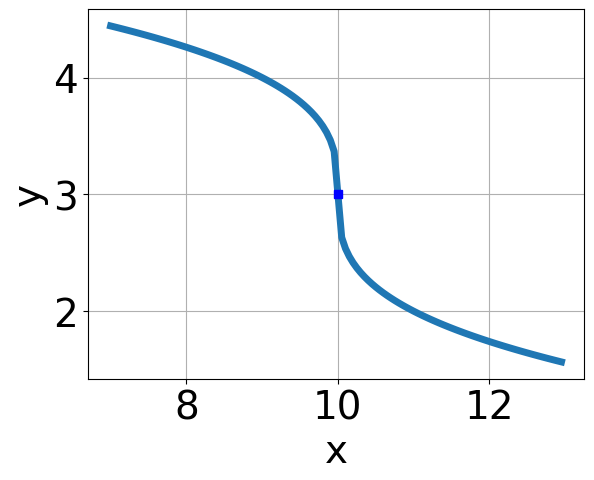
\includegraphics[width = 0.3\textwidth]{../Figures/radicalEquationToGraphAB.png}\item 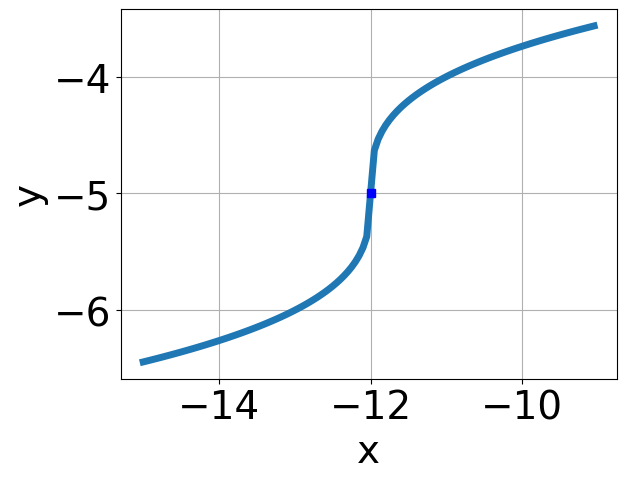
\includegraphics[width = 0.3\textwidth]{../Figures/radicalEquationToGraphBB.png}\item 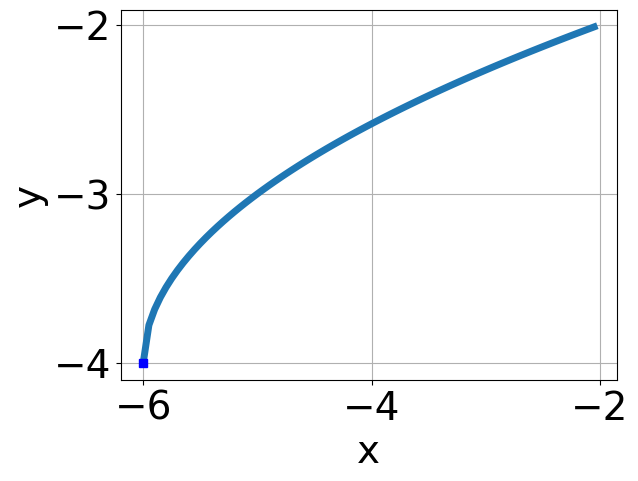
\includegraphics[width = 0.3\textwidth]{../Figures/radicalEquationToGraphCB.png}\item 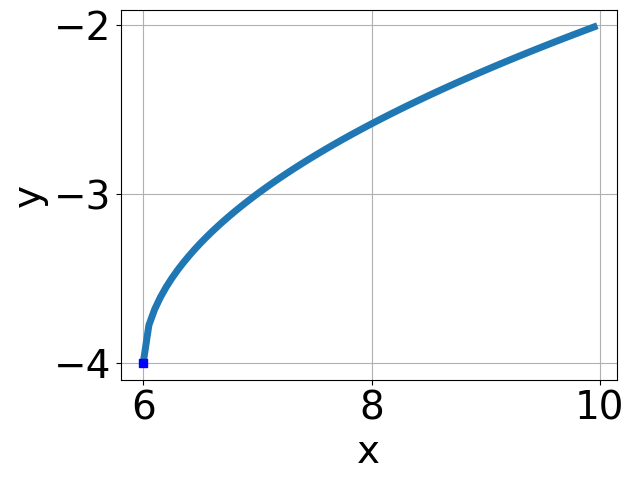
\includegraphics[width = 0.3\textwidth]{../Figures/radicalEquationToGraphDB.png}\end{multicols}\item None of the above.
\end{enumerate} }
\litem{
Choose the equation of the function graphed below.
\begin{center}
    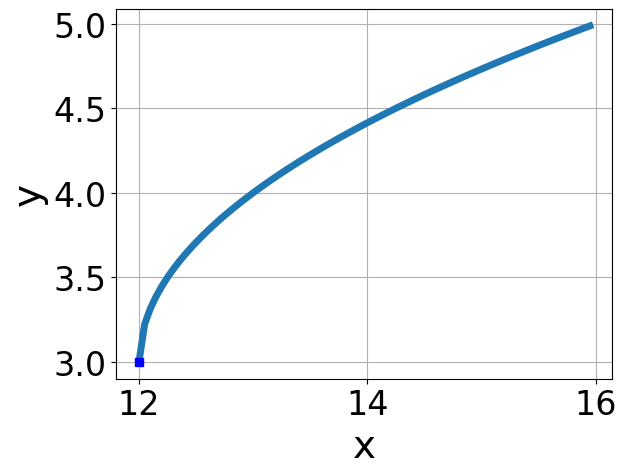
\includegraphics[width=0.5\textwidth]{../Figures/radicalGraphToEquationCopyB.png}
\end{center}
\begin{enumerate}[label=\Alph*.]
\item \( f(x) = \sqrt{x - 10} - 6 \)
\item \( f(x) = - \sqrt{x + 10} - 6 \)
\item \( f(x) = - \sqrt{x - 10} - 6 \)
\item \( f(x) = \sqrt{x + 10} - 6 \)
\item \( \text{None of the above} \)

\end{enumerate} }
\litem{
What is the domain of the function below?\[ f(x) = \sqrt[3]{-3 x - 4} \]\begin{enumerate}[label=\Alph*.]
\item \( (-\infty, \infty) \)
\item \( \text{The domain is } [a, \infty), \text{   where } a \in [-1.7, -0.94] \)
\item \( \text{The domain is } (-\infty, a], \text{   where } a \in [-0.9, 0.78] \)
\item \( \text{The domain is } [a, \infty), \text{   where } a \in [-1.3, -0.43] \)
\item \( \text{The domain is } (-\infty, a], \text{   where } a \in [-2.25, -1.15] \)

\end{enumerate} }
\litem{
Choose the equation of the function graphed below.
\begin{center}
    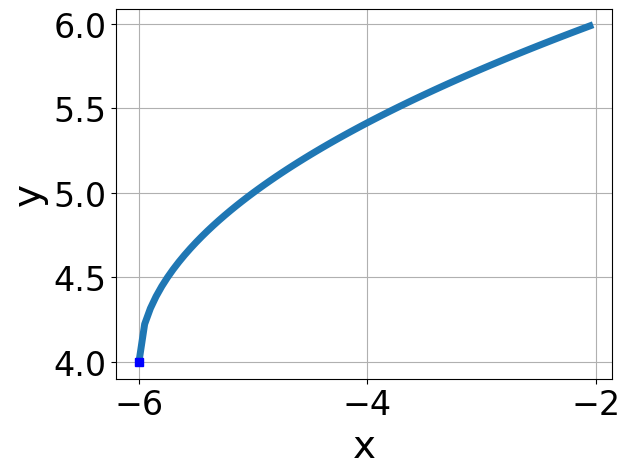
\includegraphics[width=0.5\textwidth]{../Figures/radicalGraphToEquationB.png}
\end{center}
\begin{enumerate}[label=\Alph*.]
\item \( f(x) = - \sqrt[3]{x + 12} + 5 \)
\item \( f(x) = \sqrt[3]{x - 12} + 5 \)
\item \( f(x) = - \sqrt[3]{x - 12} + 5 \)
\item \( f(x) = \sqrt[3]{x + 12} + 5 \)
\item \( \text{None of the above} \)

\end{enumerate} }
\litem{
Solve the radical equation below. Then, choose the interval(s) that the solution(s) belongs to.\[ \sqrt{45 x^2 - 56} - \sqrt{-37 x} = 0 \]\begin{enumerate}[label=\Alph*.]
\item \( x_1 \in [-4.3, -1.2] \text{ and } x_2 \in [0.09,1.18] \)
\item \( x_1 \in [-0.4, 2] \text{ and } x_2 \in [1.28,2.34] \)
\item \( x \in [-4.3,-1.2] \)
\item \( x \in [-0.4,2] \)
\item \( \text{All solutions lead to invalid or complex values in the equation.} \)

\end{enumerate} }
\litem{
Choose the graph of the equation below.\[ f(x) = \sqrt[3]{x - 14} + 6 \]\begin{enumerate}[label=\Alph*.]
\begin{multicols}{2}\item 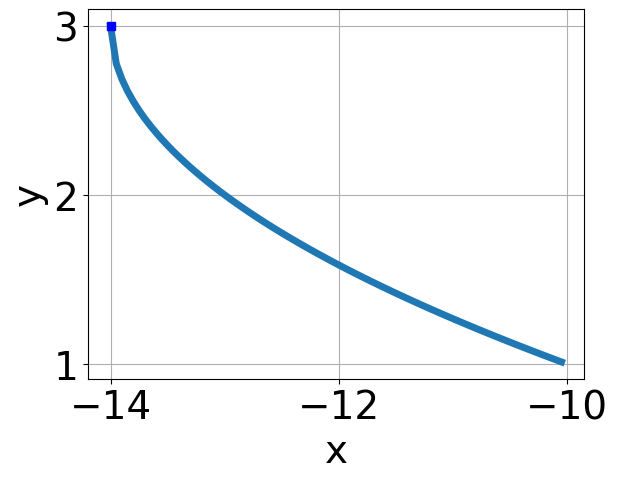
\includegraphics[width = 0.3\textwidth]{../Figures/radicalEquationToGraphCopyAB.png}\item 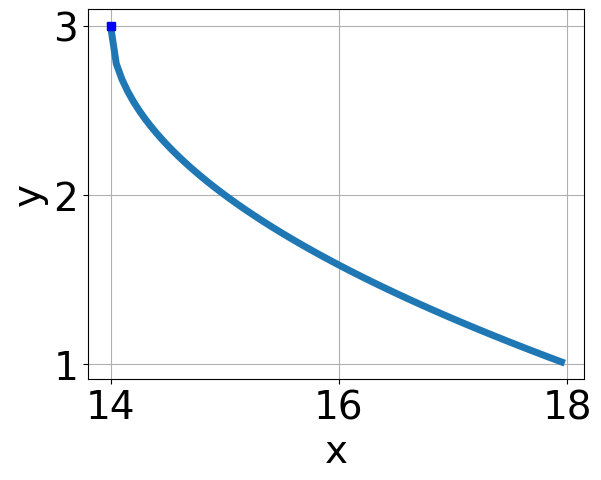
\includegraphics[width = 0.3\textwidth]{../Figures/radicalEquationToGraphCopyBB.png}\item 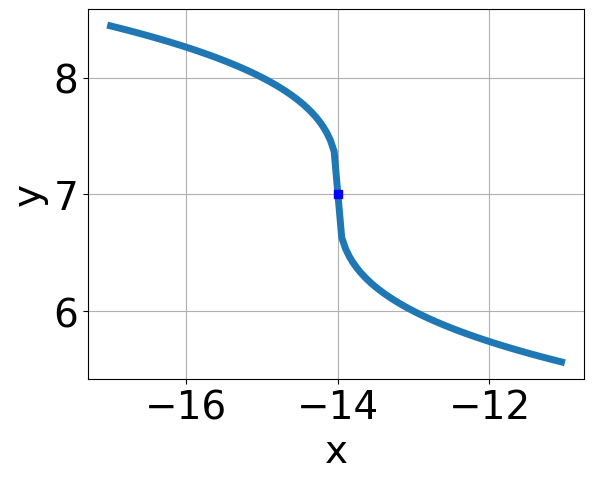
\includegraphics[width = 0.3\textwidth]{../Figures/radicalEquationToGraphCopyCB.png}\item 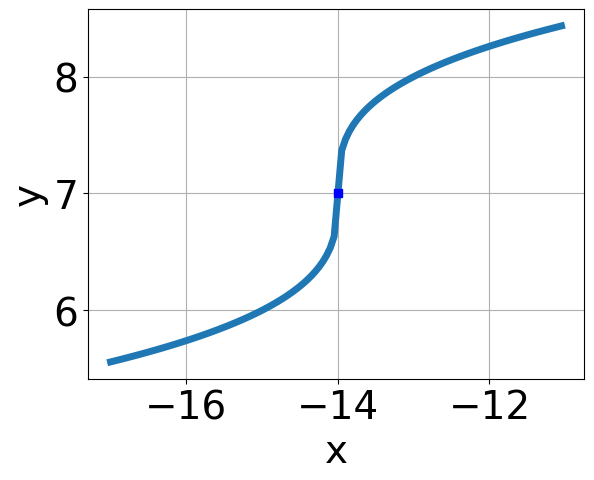
\includegraphics[width = 0.3\textwidth]{../Figures/radicalEquationToGraphCopyDB.png}\end{multicols}\item None of the above.
\end{enumerate} }
\end{enumerate}

\end{document}